% FIGURES

\begin{figure}[H]
	
	\begin{subfigure}[b]{0.48\textwidth}
		\centering
		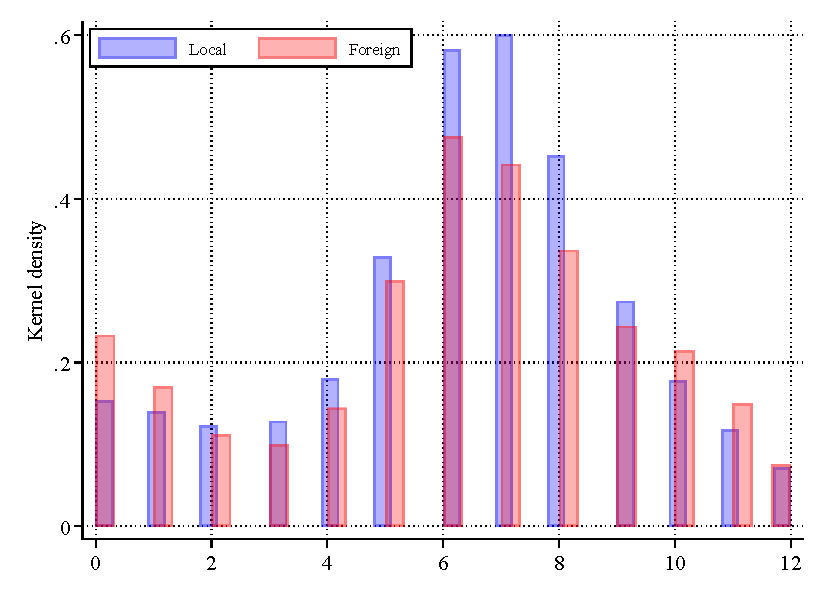
\includegraphics[width=1\linewidth]{Figures/cpi_current_N_density2}
		\caption{$\text{CPI}_t$ }
		\label{fig:cpi_current_N_density2}
	\end{subfigure}
	\hfill
	\begin{subfigure}[b]{0.48\textwidth}
		\centering
		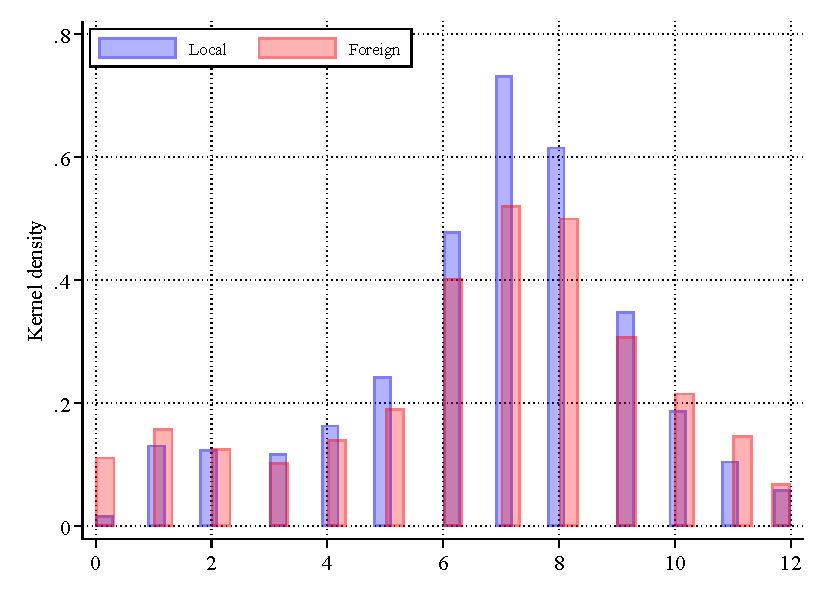
\includegraphics[width=1\linewidth]{Figures/gdp_current_N_density2}
		\caption{$\text{GDP}_t$}
		\label{fig:gdp_current_N_density2}
	\end{subfigure}
	
		\begin{subfigure}[b]{0.48\textwidth}
		\centering
		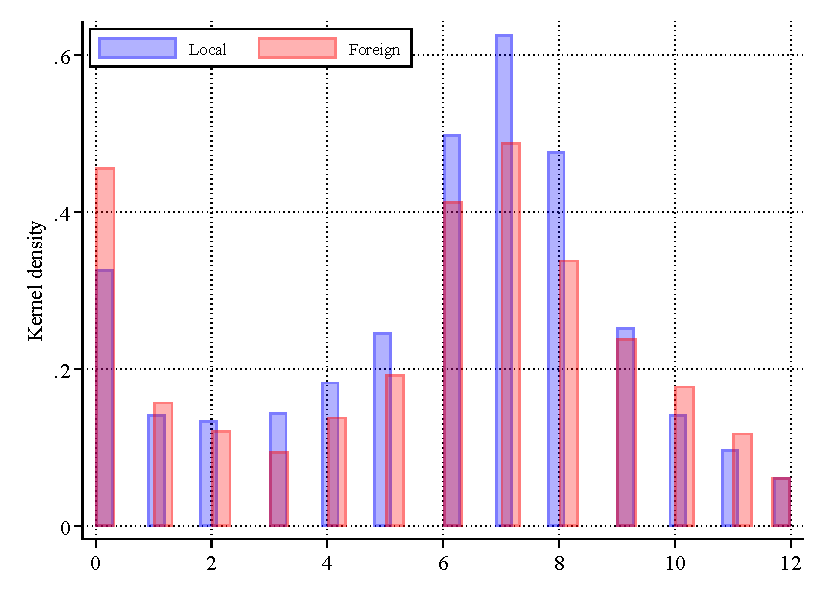
\includegraphics[width=1\linewidth]{Figures/cpi_future_N_density2}
		\caption{$\text{CPI}_{t+1}$}
		\label{fig:cpi_future_N_density2}
	\end{subfigure}
	\hfill
	\begin{subfigure}[b]{0.48\textwidth}
		\centering
		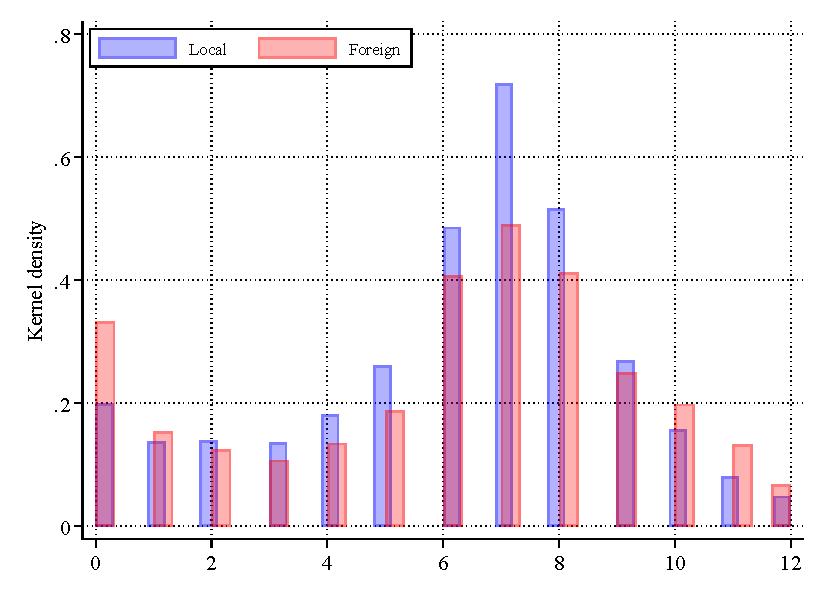
\includegraphics[width=1\linewidth]{Figures/gdp_future_N_density2}
		\caption{$\text{GDP}_{t+1}$}
		\label{fig:gdp_future_N_density2}
	\end{subfigure}
	
	\caption{Distribution of the number of yearly updates - ``Distinct'' forecasts only}
	\label{app:fig:hist_update2}
	\begin{fignote}
		\textit{Notes:} The figure displays the histograms of the number of updates by location. The population corresponds to all the country-forecaster-year units. We only consider a forecast as an update if its value differs from the last available forecast.
	\end{fignote}
\end{figure}

